\documentclass[11pt,a4paper]{report}

% Language setting
% Replace `english' with e.g. `spanish' to change the document language
\usepackage[portuges]{babel}
% Set page size and margins
% Replace `letterpaper' with `a4paper' for UK/EU standard size
\usepackage[utf8]{inputenc}
\usepackage{graphicx}
\usepackage{url}
\usepackage{enumerate}
\usepackage{color}
\usepackage{multirow}
\usepackage{array}
\usepackage[pdftex]{hyperref}
\usepackage{listings}
\usepackage{enumitem}
\definecolor{codegreen}{rgb}{0,0.6,0}
\definecolor{codegray}{rgb}{0.5,0.5,0.5}
\definecolor{codepurple}{rgb}{0.58,0,0.82}
\definecolor{backcolour}{rgb}{0.95,0.95,0.92}

\lstdefinestyle{mystyle}{
    backgroundcolor=\color{backcolour},   
    commentstyle=\color{magenta},
    keywordstyle=\color{codegreen},
    numberstyle=\tiny\color{codegray},
    stringstyle=\color{codepurple},
    basicstyle=\ttfamily\footnotesize,
    breakatwhitespace=false,         
    breaklines=true,                 
    keepspaces=true,                 
    numbers=left,                    
    numbersep=2pt,                  
    showspaces=false,                
    showstringspaces=false,
    showtabs=true
}

\lstset{style=mystyle}

\title{PLC - Trabalho Prático 1\\
	\large Grupo nº14}

\author{Simão Pedro Batista Caridade Quintela \\ (A97444) 
        \and David José de Sousa Machado \\ (A91665)
        \and Hugo Filipe de Sá Rocha \\ (A96463)
       } %autores do documento
       
\date{\today} %data

\begin{document}

	\begin{minipage}{0.9\linewidth}
        \centering
		
\includegraphics[width=0.4\textwidth]{um.jpg}\par\vspace{1 cm}
		\href{https://www.uminho.pt/PT}
		{\scshape\LARGE Universidade do Minho} \par
		\vspace{0.6cm}
		\href{https://lcc.di.uminho.pt}
		{\scshape\Large Licenciatura em Ciências da Computação} \par
		\maketitle
		
		
\includegraphics[width=0.3\linewidth]{simao.jpg}
	    
\includegraphics[width=0.3\linewidth]{david.jpg}	
        
\includegraphics[width=0.35\linewidth]{hugo.jpg}
        
		
	\end{minipage}
	
	\tableofcontents
	
	\pagebreak
	
	\chapter{Introdução}
% 
    \paragraph{}
    No âmbito da disciplina de Processamento de Linguagens e Compiladores foi-nos proposto pelo docente Pedro Rangel Henriques a realização de um trabalho prático visando colocar em prática a utilização de expressões regulares para a análise de ficheiros de texto.

    \paragraph{}
    O trabalho prático consiste na resolução de, pelo menos, um problema em cinco propostos. Analisados os problemas acabamos por resolver o problema 1 (Processador de Pessoas listadas nos Róis de Confessados) e o problema 5 (Ficheiros CSV com listas e funções de agregação).

    \paragraph{}
    Neste documento estão apresentadas as soluções utilizadas para a resolução dos problemas abordados, bem como a correspondente demonstração do funcionamento dos programas. 

    \chapter{Enunciados e Resoluções}
    \section{Processador de Pessoas listadas nos Róis de Confessados}
    \paragraph{}
    Construa agora um ou vários programas Python para processar o texto 'processos.txt' com o intuito de calcular frequências de alguns elementos (a ideia é utilizar arrays associativos para o efeito) conforme solicitado a seguir.

    \begin{enumerate}[label=\alph*)]
        \item Calcula a frequência de processos por ano (primeiro elemento da data);
        \item Calcula a frequência de nomes próprios (o primeiro em cada nome) e apelidos (o último em cada nome) por séculos;
        \item Calcula a frequência dos vários tipos de relação: irmão, sobrinho, etc.
        \item Imprimir os 20 primeiros registos num novo ficheiro de output, mas em formato JSON.
    \end{enumerate}

    \subsection{Resolução do problema}
    \paragraph{}
    Neste trabalho decidimos utilizar uma estratégia inicial semelhante em todas as alíneas que consiste em ler todas as linhas do ficheiro \textit{processos.txt} e guardá-las num array para depois poderem ser lidas na resolução das diferentes alíneas.

    \begin{enumerate}[label=\alph*.]
        \item Na resolução da alínea a. utilizamos um dicionário \textit{years} para guardar a frequência de processos por ano associando cada ano à frequência de processos. Para obtermos o ano e processo correspondente a cada linha do ficheiro utilizamos as funções \textbf{search} e \textbf{split}, e a seguinte expressão regular ([0-9]+)[:]{2}([0-9]{4}\-[0-9]{2}\-[0-9]{2}) \\
        \begin{lstlisting}[language=Python]
def processFrequency():
    years = {}

    for line in lines:
        process_and_date = re.search('([0-9]+)[:]{2}([0-9]{4}\-[0-9]{2}\-[0-9]{2})', line)
    

        if process_and_date != None:
            process = process_and_date.group(1)
            date = process_and_date.group(2)
            data_splitted = re.split(r'-', date)
            year = data_splitted[0]

        
            if year not in years:
                years[year] = 1
            else:
                years[year] += 1

    return years
        \end{lstlisting}

        \item Na resolução da alínea b. utilizamos o dicionário \textit{centurys} que tem a seguinte estrutura:
        \begin{lstlisting}[language=Python]
# this is just an example:
centurys = {
    19: {
        "First": {"Candido": 10},
        "Last":  {"Faisca": 5}
    },
    20: {
        "First": {"Ivone": 130},
        "Last":  {"Costa": 2000}
    }
    
}
        \end{lstlisting}

        \paragraph{}
        Utilizamos a expressão regular \texttt{([0-9]{4})\-([0-9]{2})\-([0-9]{2})} com a função \textbf{search} para determinar a data da linha lida.\\ Com a expressão regular \texttt{:([A-Za-z| ]+)(:)} e com a função \textbf{findall} conseguimos identificar o nome da pessoa processada, do pai e da mãe.\\Por fim, utilizando de novo a função \textbf{findall} e a expressão regular \texttt{([A-Z][A-Za-z ]+),([A-Za-z ]+). ?(?i:(Proc.[0-9]+))} conseguimos  identificar os nomes de pessoas que tiveram envolvidas noutros processos.

        \begin{lstlisting}[language=Python]
def year_to_century(year):
    return -(-year // 100)

def nameFrequency():
    centurys = {}
    for line in lines:
        date = re.search(r'([0-9]{4})\-([0-9]{2})\-([0-9]{2})' ,line)
        names_in_dots = re.findall(':([A-Za-z| ]+)(:)', line)
        names_with_procs = re.findall('([A-Z][A-Za-z ]+),([A-Za-z ]+). ?(?i:(Proc.[0-9]+))', line)
 
        names = names_in_dots + names_with_procs
    
        if date:
            year = int(date.group(1))
            century = year_to_century(year)
            if century not in centurys:
                centurys[century] = {}
                centurys[century]["First"] = {}
                centurys[century]["Last"] = {}

        for name in names:
            person_name = name[0] 
            name_splitted = re.split(" ", person_name)
            first_name = name_splitted[0]
            last_name = name_splitted[-1]
            if first_name not in centurys[century]["First"]:
                centurys[century]["First"][first_name] = 1
            else:
                centurys[century]["First"][first_name] += 1

            if last_name not in centurys[century]["Last"]:
                centurys[century]["Last"][last_name] = 1
            else:
                centurys[century]["Last"][last_name] += 1
    return centurys
        \end{lstlisting}

        \item Na resolução da alínea c utilizamos um dicionário \textit{rel\_freq} para guardar a frequência de relações existente no ficheiro de texto. 
        
        Ao analisar o ficheiro reparamos que estes dois padrões que se repetiam:\\
        \begin{enumerate}
            \item \texttt{::Filho::Pai(opcional)::Mãe(Opcional)::}\\
            \item \texttt{nome, relação de parentesco, Proc.x} \\
        \end{enumerate}

        Para identificar o padrão \texttt{(a)} usamos a função \textbf{findall} e a expressão regular \texttt{:([A-Za-z| ]+):} . De notar que, no dicionário, o \textbf{Pai} e a \textbf{Mãe} são ambos contabilizados na entrada \textbf{Progenitor} visto que em várias linhas, por vezes a ordem pela qual aparece o nome dos mesmos é trocada. Para o efeito, e para não arriscar recolher informação errada, optamos por colocá-los na mesma entrada. \\
        \\
        Para identificar o padrão \texttt{(b)}, utilizamos a função \textbf{findall} e a expressão regular \texttt{([A-Z][A-Za-z ]+),([A-Za-z ]+). ?(?i:(Proc.[0-9]+))} para identificar as restantes relações de parentesco com o processado.
    
        \begin{lstlisting}[language=Python]
def relationFrequency():
    rel_freq = {}
    rel_freq["Progenitores"] = 0
    rel_freq["Filho"] = 0

    for line in lines:
        parents_and_son = re.findall(":([A-Za-z| ]+):", line)
    
        if parents_and_son:
            parents = parents_and_son[1:]
            rel_freq["Filho"] += 1
            rel_freq["Progenitores"] += len(parents)

        relations = re.findall("([A-Z][A-Za-z ]+),([A-Za-z ]+). ?(?i:(Proc.[0-9]+))", line)
        if relations:
            for relation in relations:
                if relation[1] not in rel_freq:
                    rel_freq[relation[1]] = 1
                else:
                    rel_freq[relation[1]] += 1

    return rel_freq
        \end{lstlisting}
    

    \item Para fechar o exercício 1 falta imprimir as primeiras 20 linhas do ficheiro \textit{processos.txt} em formato JSON.
    
    Para a resolução desta alínea utilizamos duas funções, uma para recolher informação, e outra para escrever informação no ficheiro JSON pretendido.

    A função \textbf{info\_to\_json} tem como objetivo recolher informação linha a linha (assegurando-se que não lê duas vezes a mesma linha), utilizando expresões regulares mostradas anteriormente, na seguinte forma:

        \begin{lstlisting}[language=Python]
# dada a seguinte linha tem-se
# 569::1867-05-23::Abel Alves Barroso::Antonio Alves Barroso::Maria Jose Alvares Barroso::Bento Alvares Barroso,Tio Paterno. Proc.32057.   Domingos Jose Alvares Barroso,Tio Materno. Proc.32235.::

    
json_info = { 
    575::1894-11-08 :{
        "Processo": "575",
        "Data": "1894-11-08",
        "Pessoa processada": "Abel Alves Barroso",
        "Pai": "Antonio Alves Barroso",
        "Mae": "Maria Jose Alvares Barroso",
        "Tio Paterno": "Bento Alvares Barroso",
        "Tio Materno": "Domingos Jose Alvares Barroso"
    }
        \end{lstlisting}

        \begin{lstlisting}[language=Python]
def info_to_json():
    json_info = {}

    valid_lines = 0
    i = 0
    while valid_lines < 20:
        line = lines[i]

        if line != '':
            process_and_date = re.search('([0-9]+)[:]{2}([0-9]{4}\-[0-9]{2}\-[0-9]{2})', line)
            both = process_and_date.group(0)

            if both not in json_info:
                process = process_and_date.group(1)
                date = process_and_date.group(2)
            
            
                json_info[both] = {"Processo": process, "Data": date}

                son_and_parents = re.findall(':([A-Za-z| ]+)(:)', line)

                json_info[both]["Pessoa processada"] = son_and_parents[0][0]

                if len(son_and_parents) == 2:
                    json_info[both]["Mae"] = son_and_parents[1][0]
                else:
                    json_info[both]["Pai"] = son_and_parents[1][0]
                    json_info[both]["Mae"] = son_and_parents[2][0]

                relations = re.findall('([A-Z][A-Za-z ]+),([A-Za-z ]+). ?(?i:(Proc.[0-9]+))', line)
                if relations:
                    for relation in relations:
                        json_info[both][relation[1]] = relation[0]


                valid_lines+=1
    
        i+=1
    return json_info
        \end{lstlisting}

    \paragraph{}
    Posto isto, e tendo toda a informação necessária, basta utilizar a função definida por nós \textbf{write\_on\_json} para escrever toda a informação num ficheiro JSON.

    \begin{lstlisting}[language=Python]
def write_on_json():
    json_info = info_to_json()    
    f = open('res.json', 'w')

    f.write('[\n')


    for (i,entry) in enumerate(json_info):
        f.write('   {\n')
        data = json_info[entry]
        for (j, key) in enumerate(data):
            f.write(f'       \"{key}\": \"{data[key]}\"')
            
            if j == len(data)-1:
                f.write('\n')
            else:
                f.write(',\n')
            

        if i == len(json_info)-1:
            f.write('   }\n')
        else:
            f.write('   },\n')

    f.write(']\n')
    f.close()
    \end{lstlisting}
    
    \end{enumerate}

    \section{Ficheiros CSV com listas e funções de agregação}
    \paragraph{}
    Neste enunciado pretende-se fazer um conversor de um ficheiro \textbf{CSV}(\textit{Comma separated values}) para o formato \textbf{JSON}. Para se realizar a conversão pretendida, é importante saber que a primeira linha do \textbf{CSV} dado funciona como cabeçalho que define o que representa cada coluna.\\
    Por exemplo, o seguinte ficheiro "alunos.csv":
    \begin{lstlisting}[]
Numero,Nome,Curso
3162,Candido Faisca,Teatro
7777,Cristiano Ronaldo,Desporto
264,Marcelo Sousa,Ciencia Politica
    \end{lstlisting}
    Corresponde à seguinte tabela:
\begin{center}
    \begin{tabular}{||c c c||} 
    \hline
    Numero & Nome & Curso \\ [0.5ex] 
    \hline
    3162 & Candido Faisca & Teatro \\ 
    \hline
    7777 & Cristiano Ronaldo & Desporto \\
    \hline
    264 & Marcelo Sousa & Ciencia Politica \\
    [1ex] 
    \hline
    \end{tabular}
\end{center}

\item No entanto, neste trabalho, os CSV recebidos têm algumas extensões.\\

    \item \textbf{Listas}\\
    Nestes datasets, poderemos ter conjuntos de campos que formam listas. \\ \\
    \textbf{Listas com tamanho definido} 
    \paragraph{}
    No cabeçalho, cada campo poderá ter um número N que representará o número de colunas que esse campo abrange. Por exemplo, imaginemos que ao exemplo anterior se acrescentou um campo \textbf{Notas}, com \textit{N}=5 ("alunos2.csv"):

    \begin{lstlisting}[]
Numero,Nome,Curso,Notas{5},,,,,
3162,Candido Faisca,Teatro,12,13,14,15,16
7777,Cristiano Ronaldo,Desporto,17,12,20,11,12
264,Marcelo Sousa,Ciencia Politica,18,19,19,20,18
    \end{lstlisting}

Isto significa que o campo \textbf{Notas} abrange 5 colunas. (Reparem que temos de meter os campos que sobram a vazio, para o \textbf{CSV} bater certo). \\

    \item \textbf{Listas com um intervalo de tamanhos} \\\\
Para além de um tamanho único, podemos também definir um intervalo de tamanhos {N, M }, significando que o
número de colunas de um certo campo pode ir de N até M. ("alunos3.csv")
    \begin{lstlisting}[]
Numero,Nome,Curso,Notas{3,5},,,,,
3162,Candido Faisca,Teatro,12,13,14,,
7777,Cristiano Ronaldo,Desporto,17,12,20,11,12
264,Marcelo Sousa,Ciencia Politica,18,19,19,20,
    \end{lstlisting}

 \\   \item \textbf{Funções de agregação} 
    \paragraph{}
Para além de listas, podemos ter funções de agregação, aplicadas a essas listas. Veja os seguintes exemplos ("alunos4.csv" e "alunos5.csv"):
\begin{lstlisting}[]
Numero,Nome,Curso,Notas{3,5}::sum,,,,,
3162,Candido Faisca,Teatro,12,13,14,,
7777,Cristiano Ronaldo,Desporto,17,12,20,11,12
264,Marcelo Sousa,Ciencia Politica,18,19,19,20,
\end{lstlisting}

\begin{lstlisting}[]
Numero,Nome,Curso,Notas{3,5}::media,,,,,
3162,Candido Faisca,Teatro,12,13,14,,
7777,Cristiano Ronaldo,Desporto,17,12,20,11,12
264,Marcelo Sousa,Ciencia Politica,18,19,19,20,
\end{lstlisting}

\item \textbf{Resultado esperado}
\begin{lstlisting}[]
[
    {
        "Numero": "3612",
        "Nome": "Candido Faisca",
        "Curso": "Teatro"
    },
    {
        "Numero": "7777",
        "Nome": "Cristiano Ronaldo",
        "Curso": "Desporto"
    },
    {
        "Numero": "264",
        "Nome": "Marcelo Sousa",
        "Curso": "Ciencia Politica"
    }
]
\end{lstlisting}

\item No caso de existirem listas, os campos que representam essas listas devem ser mapeados para listas em \textbf{JSON} ("alunos2.csv"):

\begin{lstlisting}[]
[
    {
        "Numero": "3612",
        "Nome": "Candido Faisca",
        "Curso": "Teatro",
        "Notas": [12,13,14,15,16]
    },
    {
        "Numero": "7777",
        "Nome": "Cristiano Ronaldo",
        "Curso": "Desporto",
        "Notas": [17,12,20,11,12]
    },
    {
        "Numero": "264",
        "Nome": "Marcelo Sousa",
        "Curso": "Ciencia Politica",
        "Notas": [18,19,19,20,18]
    }
]
\end{lstlisting}

\item No caso em que temos uma lista com uma função de agregação, o processador deve executar a função associada à lista, e colocar o resultado no \textbf{JSON}, identificando na chave qual foi a função executada ("alunos4.csv"):
\begin{lstlisting}[]
[
    {
        "Numero": "3612",
        "Nome": "Candido Faisca",
        "Curso": "Teatro",
        "Notas_sum": 39
    },
    {
        "Numero": "7777",
        "Nome": "Cristiano Ronaldo",
        "Curso": "Desporto",
        "Notas_sum": 72
    },
    {
        "Numero": "264",
        "Nome": "Marcelo Sousa",
        "Curso": "Ciencia Politica",
        "Notas_sum": 76
    }
]
\end{lstlisting}
        
    \subsection{Resolução do problema}
    Na seguinte secção vamos apresentar a resolução do problema. A apresentação está estruturada da seguinte forma:\\
    \begin{enumerate}
        \item Estrutura do programa
        \item Estruturas de dados
        \item Processamento dos cabeçalhos
        \item Processamento das linhas do ficheiro
        \item Escrita do resultado em formato JSON\\
    \end{enumerate}

    \item\textbf{Estrutura do programa}
\paragraph{}
Após analisar o problema e exemplos fornecidos pelo professor, decidimos criar este conversor da seguinte forma. \\
Primeiramente será lido o ficheiro, depois vão ser processados os cabeçalhos através da criação de uma estrutura em código que espelha a estrutura do ficheiro. A seguir, a estrutura referida anteriormente será utilizada para processar as linhas do ficheiro, transformando-as e guardando-as num array.\\
Para finalizar esse array é convertido em texto no formato JSON.\\

\item\textbf{Estrutura de dados}
\paragraph{}
As estruturas de dados são um array de cabeçalhos, um array de linhas e um dicionário funções agregadoras.  \\
O array de cabeçalhos é um array de dicionários que vai guardar toda a informação dos cabeçalhos do  
ficheiro CSV e organizá-la da seguinte forma: \\
\begin{lstlisting}[language=Python]
{
    "nome":  # nome do campo do csv
    "min":   # comprimento minimo do campo caso seja uma lista
    "start": # indice inicial
    "end":   # indice final
    "aggregate_func": # nome da funcaoo a executar para agregar a lista
}
\end{lstlisting}

O array de linhas é um array de dicionários também, mas estes têm a estrutura da linha com a chave a ser um cabeçalho e o valor a ser a informação desse cabeçalho já processada.  \\
\begin{lstlisting}[language=Python]
{
    "Numero": "264",
    "Nome": "Marcelo Sousa",
    "Curso": "Ciencia Politica",
    "Notas_media": 19.0,
    "Soma_prod": 2496
}
\end{lstlisting}

O dicionário de funções agregadoras contém entradas em que a chave é o nome da função e o valor é a função em si. 

\begin{lstlisting}[language=Python]
{
    "sum": sum,
    "media": lambda x : sum(x)/len(x),
    "prod": prod
}
\end{lstlisting}

\item\textbf{Processamento de cabeçalhos}
\paragraph{}
Para processar os cabeçalhos executamos um \textbf{findall} que nos permite tornar a linha num array de tuplos  
que tem a seguinte forma (nome, intervalo de colunas, função agregadora). De seguida percorremos esse  
array e convertemo-lo na primeira estrutura mencionada anteriormente.

\begin{lstlisting}[language=Python]
def rangeToTuple(range):
    res = re.findall("(?:[0-9])+", range)
    nums = [int(num) for num in res]

    if len(nums) == 0:
        return [1, 1]
    if len(nums) == 1:
        return [1, nums[0]]
    return nums

headers = re.findall("([A-Za-z0-9@úãóíáõé]+)+({(?:[0-9]+,?)+})?(::[A-Za-z]+)?", lines[0])

# Build column structure in dictionaries
padding = 0
cols = []

for i, (nome, range, func) in enumerate(headers):
    min, max = rangeToTuple(range)
    entry = {
        "nome":  nome,
        "min":   min,
        "start": padding+i,
        "end":   padding+i+max,
        "aggregate_func": func[2:]
    }
    padding += max - 1
    cols.append(entry)
\end{lstlisting}

\item \textbf{Processamento das linhas do ficheiro}
\paragraph{}
Para processar as linhas utilizamos a estrutura criada anteriormente, verificamos que tipo de transformações  
têm de ser efectuadas para cada conjunto de colunas e preenchemos o dicionário com a informação de cada linha.  \\
\begin{lstlisting}[language=Python]
aggregators = {
    "sum": sum,
    "media": lambda x : sum(x)/len(x),
    "prod": prod
}

def rowToDict(row, cols):
    fields = re.split(",", re.sub("\n", "", row))
    dic = dict()

    for entry in cols:
        range = fields[entry["start"]:entry["end"]]

        if len(range) <= 1:
            dic[entry["nome"]] = range[0]
            continue

        converted = [int(n) for n in range if n != ""]
        if entry["aggregate_func"] == "":
            dic[entry["nome"]] = converted
        else:
            dic[f'{entry["nome"]}_{entry["aggregate_func"]}'] = aggregators[entry["aggregate_func"]](converted)

    return dic

body = lines[1:] if len(lines) > 1 else []

json = [rowToDict(row, cols) for row in body]
\end{lstlisting}


\item \textbf{Escrita do resultado em formato JSON}
\paragraph{}
Na escrita do resultado temos tabulação parametrizável e aquilo que é feito é a conversão para texto,  
utilizando \textbf{fstrings} para converter cada par do dicionário num par de JSON e o dicionário em si num objeto, depois todo esse texto é concatenado de forma a apresentar o resultado final correctamente.

\begin{lstlisting}[language=Python]
json = [rowToDict(row, cols) for row in body]

# Convert to JSON
tab = "    "

def renderPair(key, value):
    n_value = ('"' + value + '"') if type(value) is str else value
    return f'"{key}": {n_value}'

def renderObj(entry):
    outElem = f'{tab}{{\n{tab*2}'
    outElem += f',\n{tab*2}'.join([renderPair(key, value) for key, value in entry.items()])
    outElem += f'\n{tab}}}'
    return outElem

elems = [renderObj(entry) for entry in json]
out = "[\n" + ",\n".join(elems) + "\n]"


# Write result
with open("res.json", "w") as f:
    f.write(out)

\end{lstlisting}
    
    \chapter{Exemplos de funcionamento}
    \section{Processador de Pessoas listadas nos Róis de Confessados}
    \paragraph{}
    Nesta secção vamos mostrar o funcionamento do programa bem como a informação recolhida pelas funções previamente apresentadas.
    \subsection{Frequência de processos por ano}
    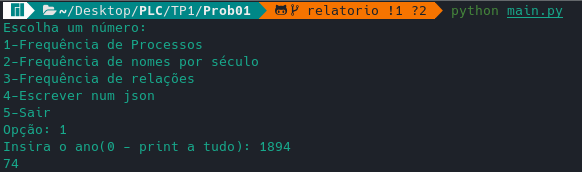
\includegraphics[width=0.8\linewidth]{alinea_a1.png} \\
	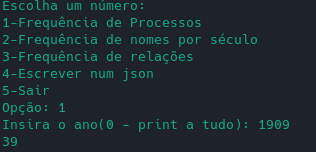
\includegraphics[width=0.8\linewidth]{alinea_a2.png}
    \paragraph{}
    Como podemos ver, o programa faz a contagem do número de processos por ano.
    
    \subsection{Frequência de nomes por século}
    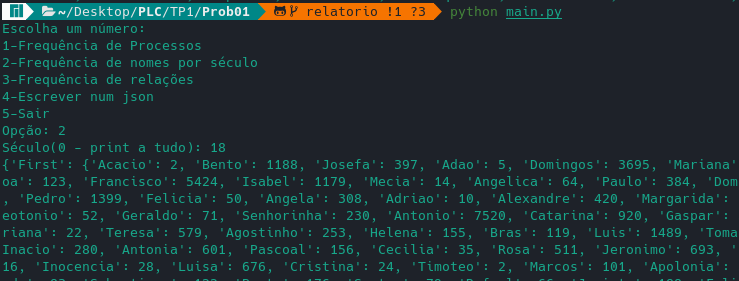
\includegraphics[width=0.8\linewidth]{alinea_b1.png} \\
	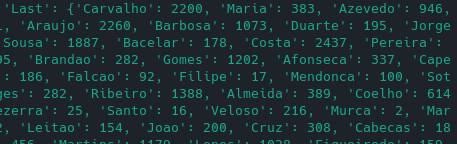
\includegraphics[width=0.8\linewidth]{alinea_b2.png}
    \paragraph{}
    Como podemos ver, o programa faz a contagem do número de nomes e apelidos por século.

    \subsection{Frequência de relações por século}
    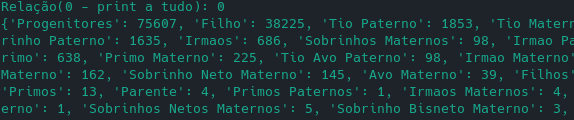
\includegraphics[width=0.8\linewidth]{alinea_c1.png} \\
    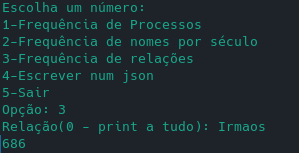
\includegraphics[width=0.8\linewidth]{alinea_c2.png}

    \paragraph{}
    Como podemos, ver o programa faz a contagem do número de relações.

    \subsection{Escrever as 20 primeiras linhas num JSON}
    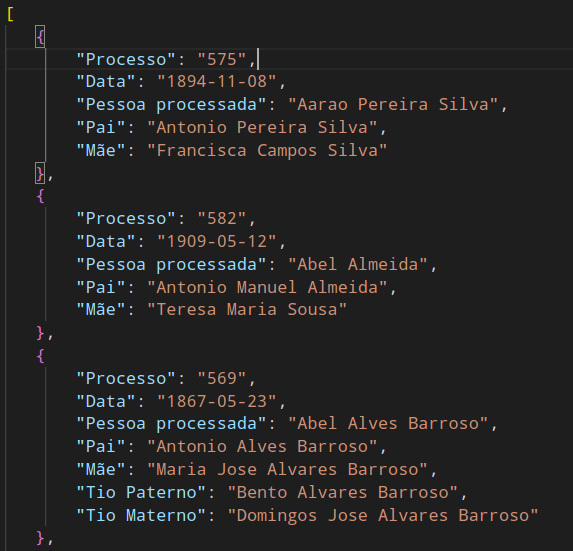
\includegraphics[width=0.8\linewidth]{alinea_d1.png} \\
    \paragraph{}
    Como podemos ver o programa está a escrever corretamente no ficheiro JSON.

\section{Ficheiros CSV com listas e funções de agregação}
    \subsection{Informação base sem listas} 
    Para o seguinte input:
\begin{lstlisting}[language=Python]
Numero,Nome,Curso
3162,Candido Faisca,Teatro
7777,Cristiano Ronaldo,Desporto
264,Marcelo Sousa,Ciencia Politica
\end{lstlisting}
Obtemos o seguinte output: \\
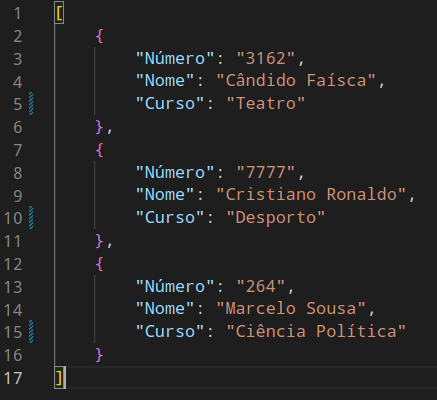
\includegraphics[width=0.8\linewidth]{prob5_1.png} \\

\subsection{Informação com listas} 
    Para o seguinte input:
\begin{lstlisting}[language=Python]
Numero,Nome,Curso,Notas{5},,,,,
3162,Candido Faisca,Teatro,12,13,14,15,16
7777,Cristiano Ronaldo,Desporto,17,12,20,11,12
264,Marcelo Sousa,Ciencia Politica,18,19,19,20,18
\end{lstlisting}
Obtemos o seguinte output: \\
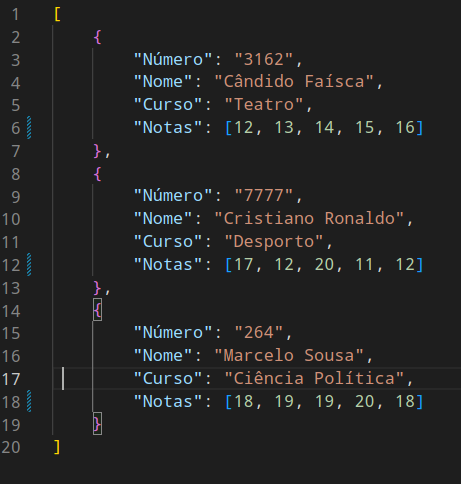
\includegraphics[width=0.8\linewidth]{prob5_2.png} \\

\subsection{Listas com um intervalo de tamanhos} 
    Para o seguinte input:
\begin{lstlisting}[language=Python]
Numero,Nome,Curso,Notas{3,5},,,,,
3162,Candido Faisca,Teatro,12,13,14,,
7777,Cristiano Ronaldo,Desporto,17,12,20,11,12
264,Marcelo Sousa,Ciencia Politica,18,19,19,20,
\end{lstlisting}
Obtemos o seguinte output: \\
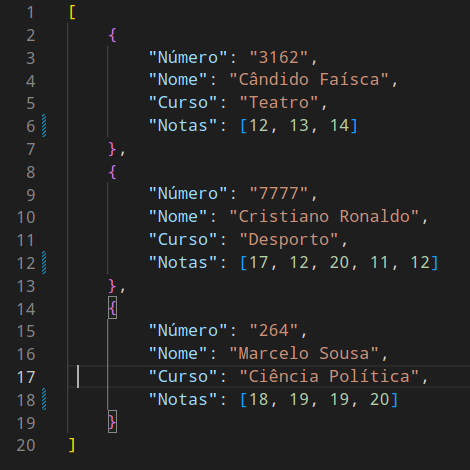
\includegraphics[width=0.8\linewidth]{prob5_3.png} \\

\subsection{Funções de agregação} 
    Para o seguinte input:
\begin{lstlisting}[language=Python]
Numero,Nome,Curso,Notas{3,5}::media,,,,,,Soma{5}::prod,,,,,
3162,Candido Faisca,Teatro,12,13,14,,,12,13,14,,
7777,Cristiano Ronaldo,Desporto,17,12,20,11,12,12,13,15,,
264,Marcelo Sousa,Ciencia Politica,18,19,19,20,,12,13,16,,
\end{lstlisting}
Obtemos o seguinte output: \\
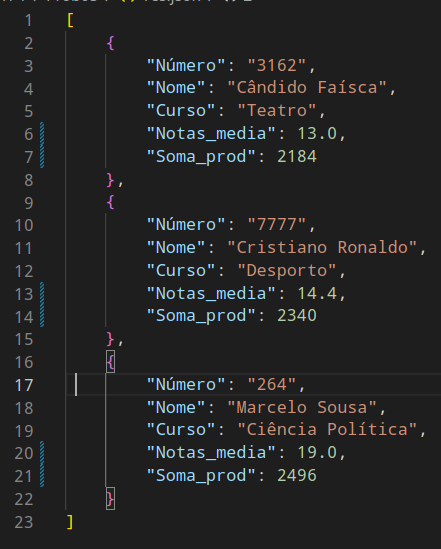
\includegraphics[width=0.8\linewidth]{prob5_4.png} \\

\chapter{Conclusão}
\paragraph{}
Fazendo uma retrospetiva referente ao trabalho prático, todos os objetivos foram cumpridos com certeza e clareza. A aposta em realizar 2 dos 5 problemas propostos fez com que todo o grupo conseguisse estar dentro do trabalho prático e adquirir todos os conhecimentos inerentes ao mesmo.
\paragraph{}
A realização deste trabalho prático fez com que entedêssemos melhor certas funções do módulo \textbf{re}, como, por exemplo, \textbf{search}, \textbf{split}, \textbf{findall} e \textbf{sub}. Também nos deu sensibilidade no que toca a lidar com ficheiros de grandes dimensões, visto que nem sempre sabíamos de que forma a informação presente nos mesmos estava formatada. 
\paragraph{}
Em suma, todos os objetivos foram concluídos sem grande dificuldade pelo grupo e consideramos que este trabalho foi uma boa preparação para o resto do semestre, no qual teremos certamente desafios nos quais utilizaremos o conhecimento aqui adquirido. 


\end{document}
